\documentclass{standalone}

\usepackage{tikz}
\usepackage{pgfplots}

\usetikzlibrary{calc}

\begin{document}
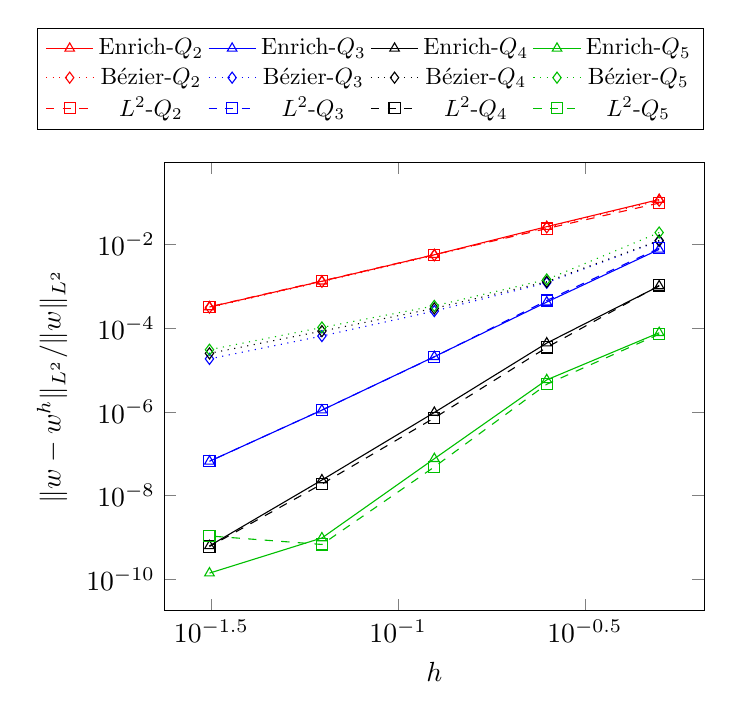
\begin{tikzpicture}
    \begin{loglogaxis}[
        legend columns=4,
    	legend style={at={(1,1.3)}, nodes={scale=.85, transform shape}},
        xlabel=$h$,
        ylabel=${\|w-w^{h}\|_{L^2}}/{\|w\|_{L^2}}$ 
    ]

    \addplot [color=red,mark=triangle] plot coordinates {

        (.5,        0.120359)
        (.25,       0.0270055)
        (.125,      0.00574049)
        (.0625,     0.00133467)
        (0.03125,   0.000322002)
    };

    
    \addplot [color=blue,mark=triangle] plot coordinates {

        (.5,        0.00771679)
        (.25,       0.000422888)
        (.125,      2.08194e-05)
        (.0625,     1.09378e-06)
        (0.03125,   6.53215e-08)
    };

    \addplot [color=black,mark=triangle] plot coordinates {

        (.5,        0.00102508)
        (.25,       4.4069e-05)
        (.125,      9.61259e-07)
        (.0625,     2.32545e-08)
        (0.03125,   6.16913e-10)
    };

    \addplot [color=green!75!black,mark=triangle] plot coordinates {


        (.5,        7.80265e-05)
        (.25,       5.81008e-06)
        (.125,      7.52504e-08)
        (.0625,     9.53475e-10)
        (0.03125,   1.37347e-10)
    };

    
    \addplot [color=red,mark=diamond, every mark/.append style={solid}, dotted] plot coordinates {

        (.5,        0.113193)
        (.25,       0.0260484)
        (.125,      0.00554975)
        (.0625,     0.00129425)
        (0.03125,   0.000312423)
    };

    
    \addplot [color=blue,mark=diamond, every mark/.append style={solid}, dotted] plot coordinates {

        (.5,        0.012241)
        (.25,       0.00122708)
        (.125,      0.000257446)
        (.0625,     6.49423e-05)
        (0.03125,   1.84527e-05)
    };

    \addplot [color=black,mark=diamond, every mark/.append style={solid}, dotted] plot coordinates {

        (.5,        0.0126067)
        (.25,       0.00129716)
        (.125,      0.000298192)
        (.0625,     8.52893e-05)
        (0.03125,   2.50418e-05)
    };

    \addplot [color=green!75!black,mark=diamond, every mark/.append style={solid}, dotted] plot coordinates {


        (.5,        0.0195279)
        (.25,       0.00146795)
        (.125,      0.000342057)
        (.0625,     0.000104338)
        (0.03125,   3.06109e-05)
    };


    \addplot [color=red,mark=square, every mark/.append style={solid}, dashed] plot coordinates {

        (.5,        0.0991881)
        (.25,       0.0243171)
        (.125,      0.00576964)
        (.0625,     0.00135489)
        (0.03125,   0.000324963)
    };

    
    \addplot [color=blue,mark=square, every mark/.append style={solid}, dashed] plot coordinates {

        (.5,        0.00825743)
        (.25,       0.000460881)
        (.125,      2.05609e-05)
        (.0625,     1.10088e-06)
        (0.03125,   6.5121e-08)
    };

    \addplot [color=black,mark=square, every mark/.append style={solid}, dashed] plot coordinates {

        (.5,        0.00105616)
        (.25,       3.46373e-05)
        (.125,      7.13333e-07)
        (.0625,     1.86819e-08)
        (0.03125,   5.94683e-10)
    };

    \addplot [color=green!75!black,mark=square, every mark/.append style={solid}, dashed] plot coordinates {


        (.5,        7.214e-05)
        (.25,       4.56071e-06)
        (.125,      4.78561e-08)
        (.0625,     6.67336e-10)
        (0.03125,   1.06707e-09)
    };

    \logLogSlopeTriangle{0.37}{0.075}{0.13}{6}{green!75!black};
    \logLogSlopeTriangle{0.16}{0.075}{0.12}{5}{black};
    \logLogSlopeTriangle{0.16}{0.075}{0.31}{4}{blue};
    \logLogSlopeTriangle{0.16}{0.075}{0.66}{2}{red};

    \legend{Enrich-$Q_2$\\Enrich-$Q_3$\\Enrich-$Q_4$\\Enrich-$Q_5$\\B\'ezier-$Q_2$\\B\'ezier-$Q_3$\\B\'ezier-$Q_4$\\B\'ezier-$Q_5$\\$L^2$-$Q_2$\\$L^2$-$Q_3$\\$L^2$-$Q_4$\\$L^2$-$Q_5$\\}
    \end{loglogaxis}
\end{tikzpicture}

\end{document}
